\subsection{Search screen}\label{subsec:search-screen}
\textbf{Opened Search screen} (Figure \ref{fig:opened_search}) is the first what a user see when he clicks on the Search button in \textbf{Dashboard}.
It shows recent results that user has searched at the last time.
The result can be a drone, aircraft, place or zone.

If a user uses \textbf{Search text field} and type a text string, it will show to him a result with an icon for better identification (Figure \ref{fig:search_results}).
If a user choose an item in the list of results, it redirects him to either to \textbf{Aircraft detail} or \textbf{Device detail}, or even a place in the map in \textbf{Dashboard}.
After choosing that item, it will appear in the list of \textbf{Recent} results.

\begin{figure}
    \centering
    \begin{minipage}{.45\textwidth}
        \centering
        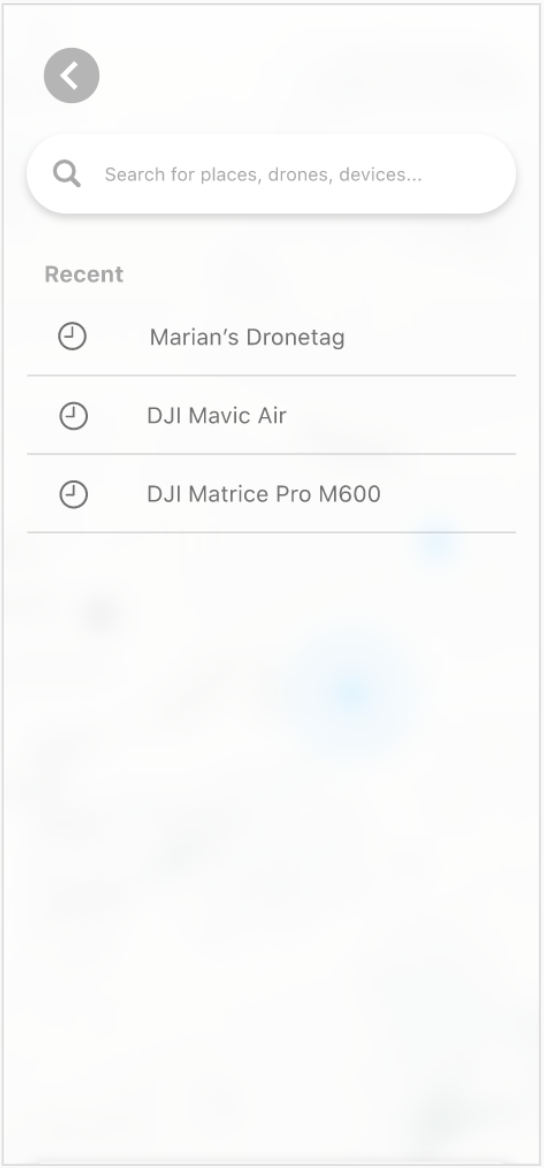
\includegraphics[width=.7\linewidth]{assets/user_interface_design/search/opened_search.png}
        \caption{[A60] Opened Search}
        \label{fig:opened_search}
    \end{minipage}%
    \hspace{.05\linewidth}
    \begin{minipage}{.45\textwidth}
        \centering
        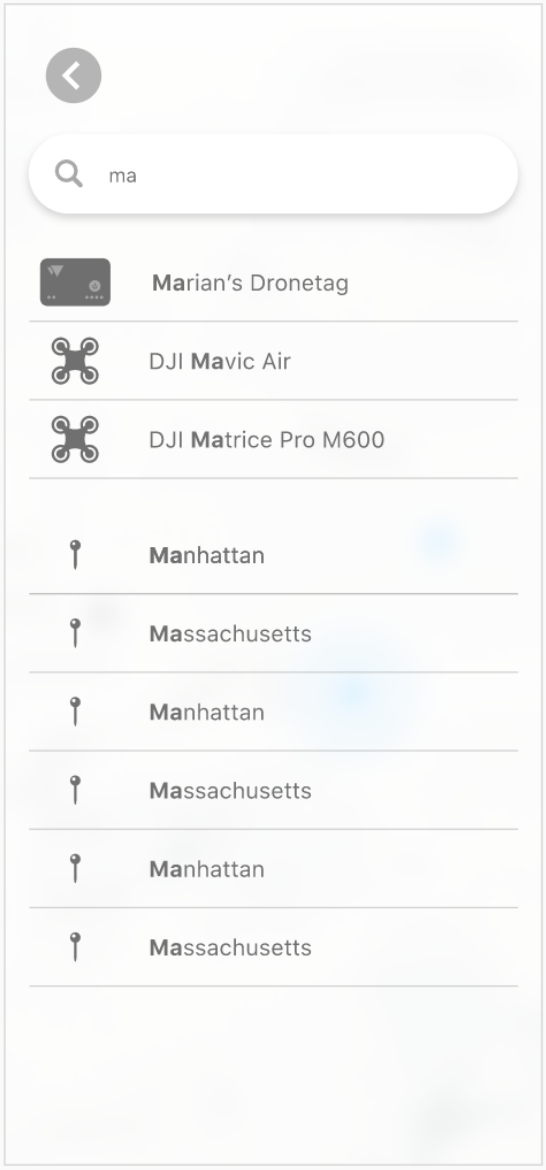
\includegraphics[width=.7\linewidth]{assets/user_interface_design/search/search_results.png}
        \caption{[A15] Search results}
        \label{fig:search_results}
    \end{minipage}
    \label{fig:search_all}
\end{figure}
